\documentclass[11pt]{report}
\usepackage[margin=2cm]{geometry}
\usepackage{graphicx}
\usepackage{hyperref}
\usepackage{amsmath}
\usepackage{amssymb}
\usepackage{upgreek}
\usepackage{amsmath,amssymb,amsthm,textcomp, stmaryrd}
\usepackage[english]{babel}
\usepackage[autostyle]{csquotes}
\usepackage[document]{ragged2e}
\usepackage{hhline}
\newcommand{\uline}[1]{\rule[0pt]{#1}{0.4pt}}

\begin{document}
\normalsize {San Quentin Math Circle // Spring 2019}

\begin{center}
	\textbf{Logic Gates}
\end{center}

\quad A \textbf{logic gate} is an idealized or physical device implementing a Boolean function; it performs a logical operation on one or more binary inputs and produces a single binary output.  Two pieces of information go in, one answer comes out.\\
\vspace{2mm}
\quad The binary number system was refined by Gottfried Wilhelm Leibniz (published in 1705), influenced by the ancient I Ching's binary system. Leibniz established that, by using the binary system, the principles of arithmetic and logic could be combined.\\
\vspace{2mm}
\quad In an 1886 letter, Charles Sanders Peirce described how logical operations could be carried out by electrical switching circuits. Eventually, vacuum tubes replaced relays for logic operations. Lee De Forest's modification, in 1907, of the Fleming valve can be used as a logic gate. Ludwig Wittgenstein introduced a version of the 16-row truth table as proposition 5.101 of Tractatus Logico-Philosophicus (1921). Walther Bothe, inventor of the coincidence circuit, got part of the 1954 Nobel Prize in physics, for the first modern electronic AND gate in 1924. Konrad Zuse designed and built electromechanical logic gates for his computer Z1 (from 1935–38).\\
\vspace{2mm}
\quad From 1934 to 1936, NEC engineer Akira Nakashima introduced switching circuit theory in a series of papers showing that two-valued Boolean algebra, which he discovered independently, can describe the operation of switching circuits.  His work was later cited by Claude E. Shannon, who elaborated on the use of Boolean algebra in the analysis and design of switching circuits in 1937. Using this property of electrical switches to implement logic is the fundamental concept that underlies all electronic digital computers. Switching circuit theory became the foundation of digital circuit design, as it became widely known in the electrical engineering community during and after World War II, with theoretical rigor superseding the ad hoc methods that had prevailed previously.\\
\vspace{2mm}
\quad Logic gates can also be used to store data. A storage element can be constructed by connecting several gates in a "latch" circuit. More complicated designs that use clock signals and that change only on a rising or falling edge of the clock are called edge-triggered "flip-flops". Formally, a flip-flop is called a bistable circuit, because it has two stable states which it can maintain indefinitely. The combination of multiple flip-flops in parallel, to store a multiple-bit value, is known as a register. When using any of these gate setups the overall system has memory; it is then called a sequential logic system since its output can be influenced by its previous state(s), i.e. by the sequence of input states. \\
\vspace{2mm}
\quad Active research is taking place in molecular logic gates.
\vspace{2mm}


\pagebreak

\begin{center}
	Let's start with the 3 fundamental logic gates: \text{\emph{AND}}, \text{\emph{OR}}, and  \text{\emph{NOT}}. \\Below is a visual representation of each operator.  Please fill out the \textbf{TRUTH TABLE} below it.
\end{center}


\vspace{20mm}
\hspace{1in}
\begin{minipage}{.5\linewidth}
	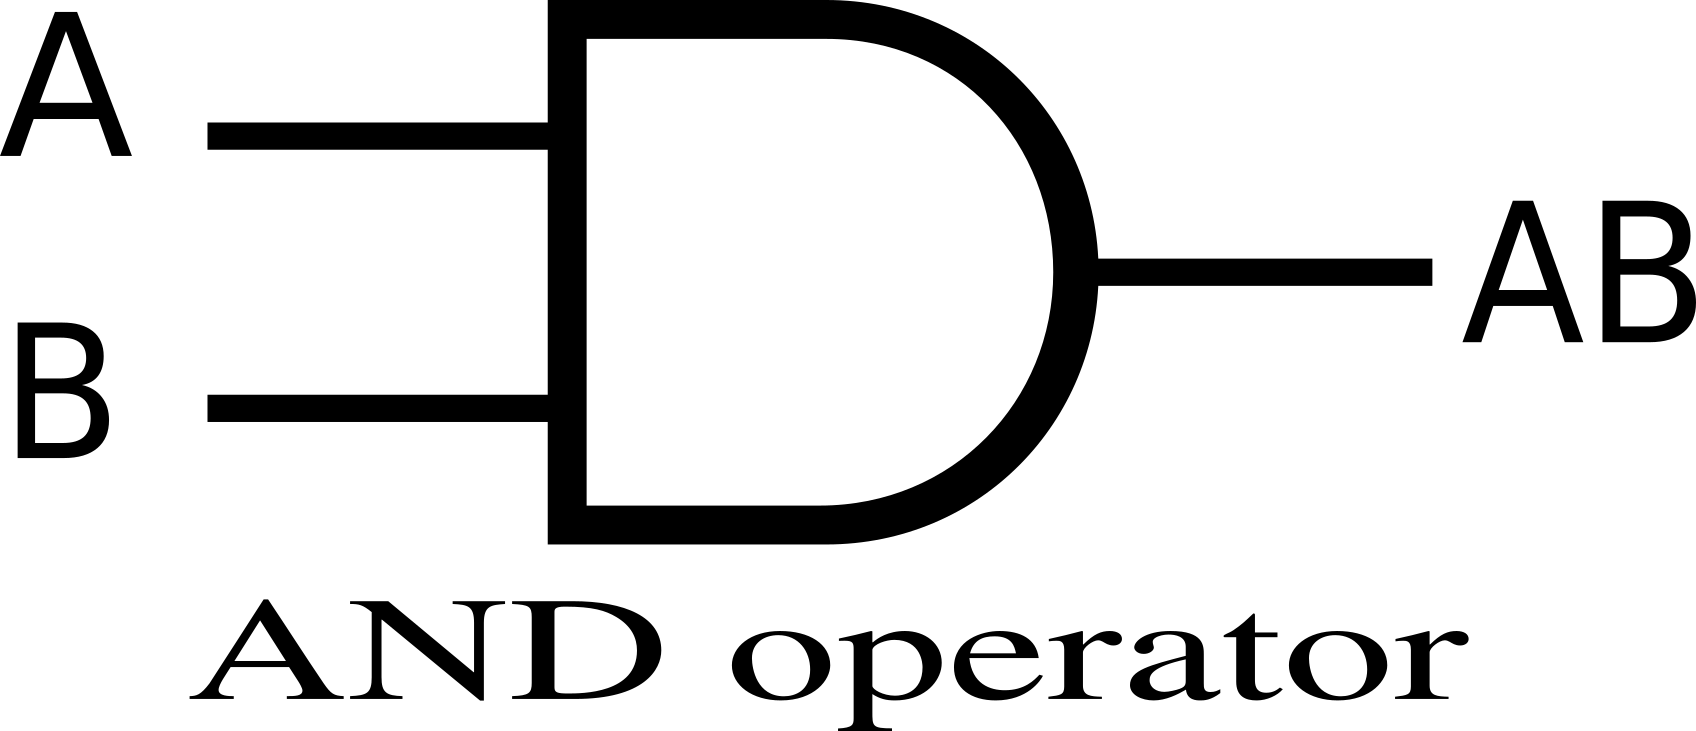
\includegraphics[width=3 in]{and.png}
	\label{img2}
\end{minipage}
\begin{minipage}{\linewidth}
\begin{tabular}{|ll|l|}
	\hline
	Input                   &   & Output  \\ \hline
	\multicolumn{1}{|l|}{A} & B & A and B \\ \hline
	\multicolumn{1}{|l|}{}  &   &         \\ \hline
	\multicolumn{1}{|l|}{}  &   &         \\ \hline
	\multicolumn{1}{|l|}{}  &   &         \\ \hline
	\multicolumn{1}{|l|}{}  &   &         \\ \hline
\end{tabular}
\end{minipage}


\vspace{20mm}
\hspace{1in}
\begin{minipage}{.5\linewidth}
	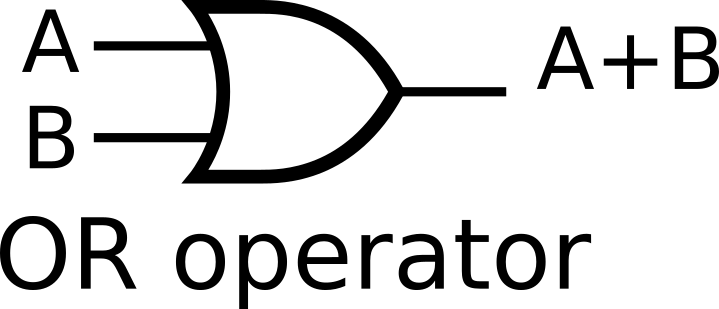
\includegraphics[width=3 in]{or1.png}
	\label{img2}
\end{minipage}
\begin{minipage}{\linewidth}
\begin{tabular}{|ll|l|}
	\hline
	Input                   &   & Output \\ \hline
	\multicolumn{1}{|l|}{A} & B & A or B \\ \hline
	\multicolumn{1}{|l|}{}  &   &        \\ \hline
	\multicolumn{1}{|l|}{}  &   &        \\ \hline
	\multicolumn{1}{|l|}{}  &   &        \\ \hline
	\multicolumn{1}{|l|}{}  &   &        \\ \hline
\end{tabular}

\end{minipage}


\vspace{20mm}
\hspace{1in}
\begin{minipage}{.5\linewidth}
	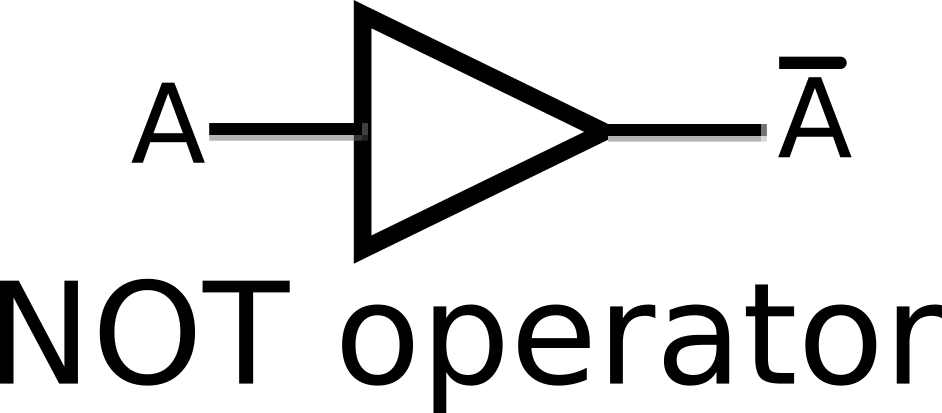
\includegraphics[width=3 in]{not1.png}
	\label{img2}
\end{minipage}
\begin{minipage}{\linewidth}
	\begin{tabular}{|l|l|}
		\hline
		Input & Output \\ \hline
		A     & NOT A  \\ \hline
		&        \\ \hline
		&        \\ \hline
	\end{tabular}
\end{minipage}


\vspace{10mm}
\begin{center}
	\Large
	\textbf{Commonly Used Symbols}
	\normalsize
	
	A and B $\rightarrow$ A $\wedge$ B or A $\cdot$ B\\
	A or B $\rightarrow$ A $\vee $ B or A + B\\
	Not A $\rightarrow$ $\bar{A}$ or $\neg$ A\\
\end{center}










\end{document}